\documentclass{article}
\usepackage[scaled]{helvet}
\renewcommand\familydefault{\sfdefault} 
\usepackage[T1]{fontenc}
\usepackage{subcaption}
\usepackage{float}
\usepackage{fancyhdr}
\usepackage{graphicx}
\usepackage{subfigure}
\usepackage{booktabs}
\usepackage[inline]{enumitem}

\usepackage{amsmath}

\usepackage{hyperref}
\hypersetup{
    colorlinks=true,
    citecolor=[RGB]{0,0.5,0.5},
    urlcolor=[RGB]{0,0.5,0.5},
    linkcolor=[RGB]{0,0.5,0.5}
}

\usepackage{geometry}
\geometry{margin={0.2in,0.2in}}

\usepackage[colorinlistoftodos,prependcaption,textsize=small]{todonotes}

\begin{document}

\begin{centering}
\Large\textbf{\sc Acoustic Signal Classification Informal Report}\\[0.5ex]
{Kanwar Pannu}\\
\vspace{0.1in}
\end{centering}
\hrule


% This is the template your should use for your project report.
% \autoref{fig:formulas} provides an example of how figures are typeset in Latex.
% Feel free to modify the text of this document as you like.
% You can also insert figures and tables for reporting the model's performance.
% Please keep the overall template
% \begin{figure}[h!]
%     \centering
%     \subfigure[
%         ``$2 + 0$''
%     ]{
%         \label{fig:formula-0}
%         \includegraphics[scale=1]{figure/formula_000.png}
%     }
%     \subfigure[
%         ``$5 + 6$''
%     ]{
%         \label{fig:formula-1}
%         \includegraphics[scale=1]{figure/formula_001.png}
%     }
%     \subfigure[
%         ``$2 \cdot 9$''
%     ]{
%         \label{fig:formula-2}
%         \includegraphics[scale=1]{figure/formula_002.png}
%     }
%     \subfigure[
%         ``$4 - 1$''
%     ]{
%         \label{fig:formula-3}
%         \includegraphics[scale=1]{figure/formula_003.png}
%     }
%     \subfigure[
%         ``$3 / 3$''
%     ]{
%         \label{fig:formula-4}
%         \includegraphics[scale=1]{figure/formula_004.png}
%     }
%     \caption{
%         Figure captions are inserted here.
%     }
%     \label{fig:formulas}
% \end{figure}

\section{Introduction}
This is an informal report for the acoustic signal classification project. The goal of this project is to classify acoustic signals using machine learning techniques into "Drummy" or "Tight". The dataset used for this project is divided into 2 phases: Phase 1 and Phase 2.

\section{Stage 1}
\subsection{Data Analysis}
\subsubsection{Phase 1}
Phase 1 consists of \textbf{3,309 recordings} (\textbf{2,212 drummy} sounds and \textbf{1,097 tight sounds}).
Recordings in this phase have a duration of \textbf{0.75 seconds} and \textbf{36000 samples per recording}. The recordings are sampled at a rate of \textbf{48 kHz}. The dataset is not balanced, with number of drummy sounds twice that of tight sounds.
\paragraph{Findings}
\begin{itemize}
    \item Did a quick PCA analysis (first standardizing the data) and plotted the first 2 principal components. The 3D scatter plot (PC1 vs PC2 vs Label) shows that drummy and tight sounds are not linearly separable, and that tight sounds form a cluster in the middle of drummy sounds, while drummy sounds are more spread out.
    \begin{figure}[h!]
        \centering
        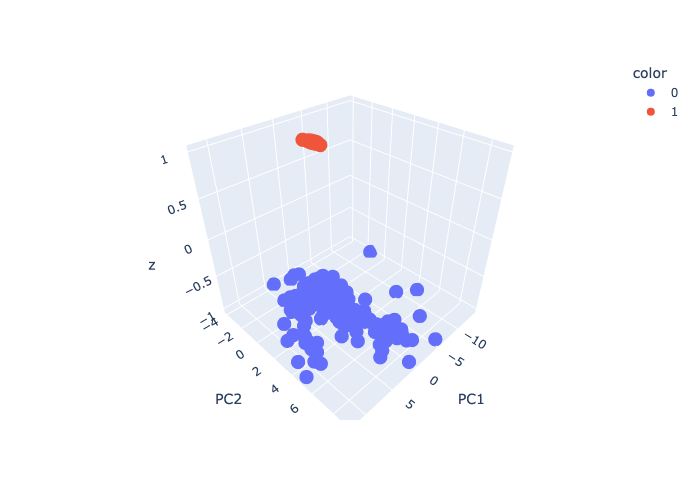
\includegraphics[width=0.4\textwidth]{../assets/p1_pca_3d.png}
        \caption{2 Component PCA Analysis of Phase 1 Data}
        \label{fig:phase1_pca_2_comp}
    \end{figure}
    \item Waveform visualization shows that drummy sounds dampen relatively slowly and have a longer decay time, while tight sounds dampen quickly and have a shorter decay time.
    \begin{figure}[H]
        \centering
        \begin{subfigure}{0.4\textwidth}
            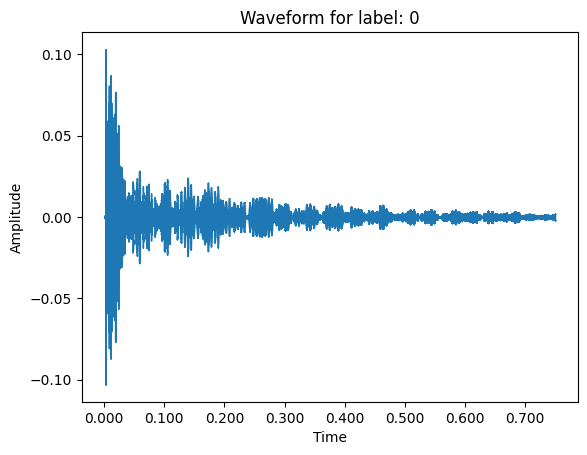
\includegraphics[width=\textwidth]{../assets/p1_waveform_0.png}
            \caption{Drummy Waveform Visualization (Phase 1)}
            \label{fig:phase1_waveform_0}
        \end{subfigure}
        \hfill
        \begin{subfigure}{0.4\textwidth}
            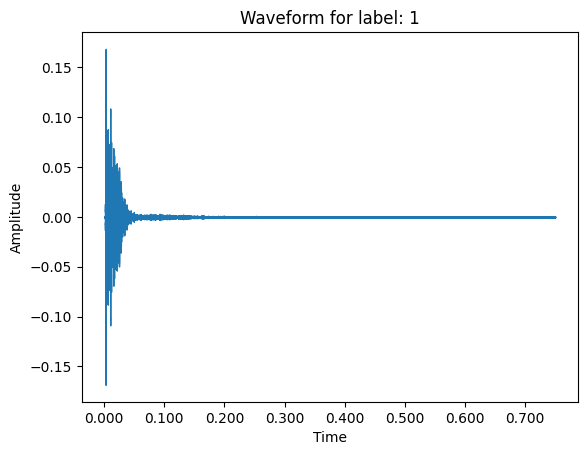
\includegraphics[width=\textwidth]{../assets/p1_waveform_1.png}
            \caption{Tight Waveform Visualization (Phase 1)}
            \label{fig:phase1_waveform_1}
        \end{subfigure}
        \caption{Waveform visualizations for different drum styles in Phase 1}
        \label{fig:phase1_waveforms}
    \end{figure}
    \item S
\end{itemize}
\subsubsection{Phase 2}
Phase 2 consists of \textbf{9,923 recordings} (from which \textbf{1,483} recordings were \textbf{corrupted with NaN value}s, making it 8,440 recordings; further, there are \textbf{some mis-hits} as well that need to be cleaned later for feature extraction to be done on them). Finally, there are \textbf{3,856 drummy sounds and 3,124 tight sounds (including the mis-hits)}. Each recording has 4800 samples and a duration of \textbf{0.1 seconds}. The recordings are sampled at a rate of \textbf{48 kHz}. The dataset is more balanced than Phase 1, with number of drummy sounds slightly higher than tight sounds.

\end{document}